%-----------------------------------------------------------------------------------------------------------------
%% Section 1
\chapter{Question 1: Mass Actuator System}
\label{chap:q1}

As per \cite{assign}, it is required to find the natural frequency $\omega_n$ of the mass actuator system in Figure~\ref{fig:q1} below.

\begin{figure}[H]
	\centering
	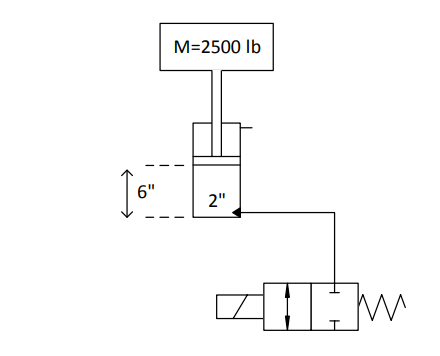
\includegraphics[scale=1]{q1}
	\caption{Schematic for question 1.}
	\label{fig:q1}
\end{figure}

From this, applying newtons second law \ref{eq:q1_newt}.

\begin{equation}
	\label{eq:q1_newt}
	m \ddot{y} = f(t) - b\dot{y} - k y
\end{equation}

Taking the Laplace of the above functions with zero initial conditions
\begin{equation}
	ms^2 Y(s) + b s Y(s) + k Y(s) = F(s)
\end{equation}

Rearranging
\begin{equation}
	\label{eq:q1_tfactual}
	T(s) = \frac{Y(s)}{F(s)} = \frac{\frac{1}{m}}{s^2 + \frac{b}{m}s + \frac{k}{m}}
\end{equation}



Compared to desired second order transfer functions $H(s)$ \ref{eq:q1_tfideal}.
\begin{equation}
	\label{eq:q1_tfideal}
	T(s)= \frac{X(s)}{F(s)} = \frac{\omega_n^2}{s^2+2\zeta\omega_n s + \omega_n^2}
\end{equation}


From this

\begin{equation}
	\label{eq:q1_wn}	
	\omega_n = \sqrt{\frac{k}{m}}	
\end{equation}

Therefore need fluid equivalent of k.

\begin{equation}
	\label{eq:q1_beta}
	\beta = - \frac{\Delta p V_0}{\Delta V}	
\end{equation}

Realizing that $V_0 = AL$ and $\Delta V = Ax$, solving for $\Delta p$ yields the following

\begin{equation}
	\label{eq:q1_f}
	\Delta p = \frac{F}{A}= \beta \ \frac{y}{l} \Rightarrow F = \frac{A\beta}{l}y 	
\end{equation}

Knowing that $F = ky$ comparing the result of \ref{eq:q1_f} yields the final relation for the equivalent stiffness $k$

\begin{equation}
	\label{eq:q1_k}
	 k = \frac{A\beta}{l} 	
\end{equation}


